\documentclass[a4paper,10pt]{article}
\usepackage[utf8]{inputenc}
\usepackage{graphicx}

% Title Page
\title{RaCa-Engine}
\author{Martin Yrjölä}


\begin{document}
\maketitle

\section{Personal Information}

Martin Yrjölä\newline
84086N\newline
TIK I\newline

\section{Description}

A simple 3D rendering engine using the Java Swing library. The environment
consists off a plane with solid walls aligned in a grid. You are able to move in
the plane, but collide with walls. The technique used for the rendering is
called ray-casting, a subclass of ray tracing. The after-mentioned could be
shortly described as tracing rays of light from the viewers eye to the object in
the scene. Ray-casting is simpler and faster. You cast only one ray for every
vertical strip on the screen. The walls are textured and shaded darker the
further they are from the viewer. The environment is made in a level-editor,
which is an integral part of the application. For example it can be
invoked when the rendering is running and the environment can be edited in
real-time. There is options available for the user through a settings file. The
field-of-view, number of rays cast and display resolution as a few examples of
the available options. The project is implemented conforming to the hard
difficulty specification.

\section{Usage Manual}

\subsection{Setting up}
The settings.ini file in the base directory contains the options. If it's
missing you can generate a new one by running the program. An option consists
of a key and value pair separated with a colon ':'. There's no correct value
checking for settings, so things can break. For example setting FOV to 180
causes division by zero and crashes the program. Changing settings is not
fool-proof and is considered an experimental feature. If you break something
just delete the file and let the program generate a new one. The settings are as
follows:

\begin{itemize}
\item MS\_PER\_TICK: The time between engine logic (movement, AI, physics...) 
updates in milliseconds.
\item MAX\_FPS: Sets maximum Frames Per Second.
\item KEY\_UP: The keycode for moving forward.
\item KEY\_DOWN: The keycode for backwards movement.
\item KEY\_RIGHT:The keycode for turning right.
\item KEY\_LEFT: The keycode for turning left.
\item KEY\_LOOK\_UP: The keycode for looking up.
\item KEY\_LOOK\_DOWN: The keycode for looking down.
\item KEY\_STRAFE\_LEFT: The keycode for strafing left.
\item KEY\_STRAFE\_RIGHT: The keycode for strafing right.
\item SHOW\_FPS: Show Frames Per Second 0 = false , 1 = true.
\item RESOLUTION\_X: The horizontal resolution.
\item RESOLUTION\_Y: The vertical resolution.
\item VIEW\_DISTANCE: The view distance in grids before the shading begins.
\item GRID\_SIZE: The size of one square in the grid.
\item FOV: Field Of View in degrees.
\item PIXELS\_PER\_SQUARE: The number of pixels representing a square in
the level editor.
\item WALL\_TEXTURES: Number of different textures for the walls. Found in
res/wall\{numbers from 1 to 9\}.png. If set to zero no textures will be used.
The walls will be drawn white.
\end{itemize}

\subsection{Running the level editor}
First make sure you're in the base directory and run the application with:
\begin{verbatim}
 java -classpath src/ leveleditor.LevelEditor
\end{verbatim}

\subsection{Using the level editor}

\subsubsection{The user interface}

\begin{figure}[h]
 \centering
 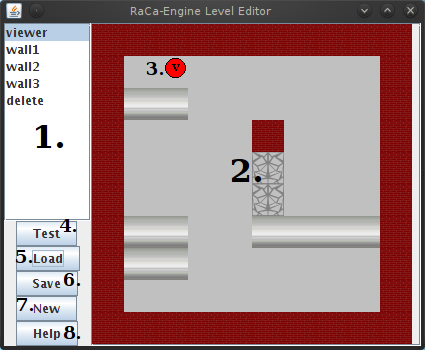
\includegraphics{leveleditor_screenshot.png}
 % leveleditor_screenshot.png: 425x350 pixel, 93dpi, 11.61x9.56 cm, bb=0 0 329
271
\end{figure}

\begin{enumerate}
 \item Object list. Choose an object from here and it will be placed where
you click in the map view. Except for delete, which will clear the clicked
square.
\item Map view. Click here to place/delete objects.
\item Viewer. The movable camera. There can only be one viewer at a time in the
map view.
\item Test button. Launches the engine in the levels current state. Some
buttons are disabled, but the map view still works. So the level can be edited
in real-time. To end the rendering just close the engine's window.
\item Loads a new level in a file choosing dialog.
\item Saves the current level in levels/\{level number\}.lvl.
\item New Level button. Opens a dialog to create a new level.
\item The help button displays the mapped keys in human readable form.
\end{enumerate}

\subsubsection{The new level dialog}

\begin{figure}[h]
 \centering
 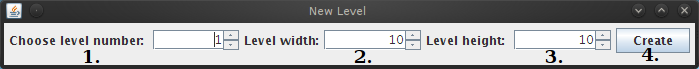
\includegraphics[scale=0.60]{new_level_screenshot.png}
 % new_level_screenshot.png: 699x69 pixel, 93dpi, 19.09x1.88 cm, bb=0 0 541 53
\end{figure}

\begin{enumerate}
\item Determines in which file the level will be saved.
\item Determines how many squares wide the level is.
\item Determines how many squares high the level is.
\item Creates the level with the chosen settings and opens it in the editor.
\end{enumerate}

\subsection{The engine}

\begin{figure}[h!]
 \centering
 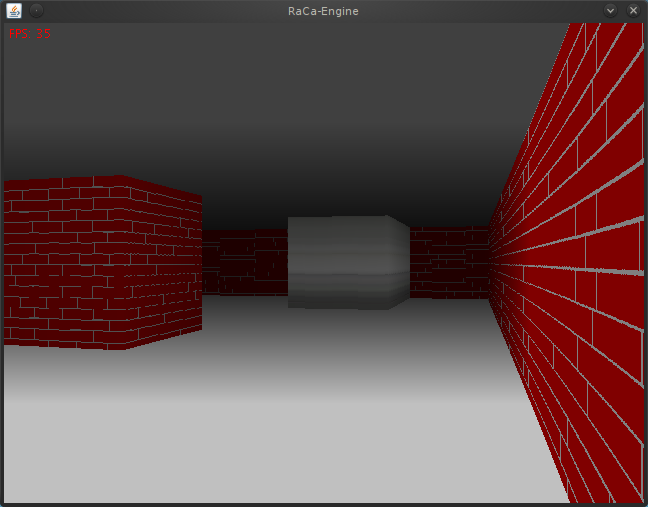
\includegraphics[scale=0.65]{engine_screenshot.png}
 % engine_screenshot.png: 648x507 pixel, 93dpi, 17.70x13.85 cm, bb=0 0 502 393
\end{figure}

After pressing the test button you get to the engine. The default keys are:

\begin{itemize}
 \item Up arrow to move forward.
\item Down arrow to move backward.
\item Left arrow to turn left.
\item Right arrow to turn right.
\item 'W' to look up.
\item 'S' to look down.
\item 'A' to strafe left.
\item 'D' to strafe right.
\end{itemize}

Just move around in the world you created and observe that you can still edit
the level while the engine is running. To exit just close the window.

\section{Structure}

I chose to use the Model-View-Controller pattern for this project. I had already
decided to separate rendering from the rest of the logic(movement,
collision-detection, etc.) and considered the usage of a design pattern to
clarify the framework. MVC also separates the data (Model) from the manipulator
(Controller), so it should provide even more flexibility. E.g. the viewpoint
could be controlled by keyboard and switched to AI or mouse control only by
switching the Controller.

I had thought of skipping the Controller part and let the Entities themselves
handle input-control and collision detection. This is what many games do,
because it's easier to handle many instances. My engine won't have hordes of
actors on the screen so the MVC-pattern was motivated for more flexible control

There exists javadoc documentation for the project and therefore I instruct the
reader to consult it when looking at the structure of the project. The
index.html lies in the javadoc directory.

A rough separation is as follows: The model lies in the environment package,
The controllers are in controllers and the view is in renderer.

\section{Algorithms and mathematical formulas}
The walls are aligned in a grid. Therefore to calculate the distance to a wall I
only need to check for walls between the grids. So there's a check for both
horizontal and vertical walls. To get the first intersection I only have to
round to the nearest multiple of grid width taking the directions quadrant into
consideration.
\begin{figure}[h!]
 \centering
 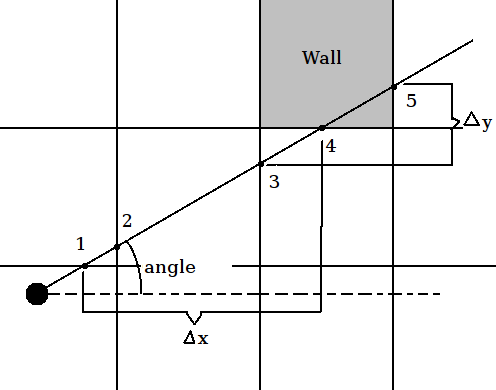
\includegraphics[scale=0.85]{find_wall.png}
 % find_wall.png: 496x390 pixel, 93dpi, 13.55x10.65 cm, bb=0 0 384 302
\end{figure}
\begin{center}
$\triangle x=\frac{grid\: height}{\tan(angle)}$, $\triangle y=grid\:
width*\tan(angle)$
\par\end{center}

After I find the position of the wall the distance is computed by the following
formulas:


\begin{itemize}
\item If there was a wall on a vertical grid:
\end{itemize}
\begin{center}
$distance=abs(\frac{viewerX-collisionX}{cos(direction)})$\\

\par\end{center}
\begin{itemize}
\item For horizontal walls the formula looks like this:
\end{itemize}
\begin{center}
$distance=abs(\frac{viewerY-collisionY}{sin(direction)})$\\
\par\end{center}

\subsection{Distance correction}

Now the walls are projected on a flat surface. This is okay for a
screen. But it's not how the human eye sees things because its round.
The distortion is corrected by the following formula:

\begin{center}
$corrected\: distance=distorted\: distance*\cos(angle)$\\

\par\end{center}

\subsection{Interpolation}

The engine will update it's logic at fixed rate and visuals at variable
FPS. This means frames will also be rendered between ticks. So the
renderer must predict where an entity is going to be for a smoother
experience on fast hardware. The formula looks like:

\begin{center}
$prediction=position+(speed+acceleration)*interpolation$
\par\end{center}

\begin{center}
$interpolation=\frac{time\: to\: next\: tick}{time\: between\: ticks}$\\
\par\end{center}

\subsection{Rendering}

In pseudocode the screen is rendered like this:

\begin{verbatim}
1. Draw shaded floor and ceiling in the background.
2. Cast rays to determine distances to walls.
3. Draw the correct part of texture to each strip.
4. Update the shade factor for each strip.
5. Draw the strips to the screen buffer scaling them to correct height and using
the given shade factor.
6. Update the screen.
\end{verbatim}

\section{Data Structures}

\subsection{World}

The world is represented by a two-dimensional matrix
char{[}height{]}{[}width{]}. So the world is grid-based. This makes it much more
effective to check where a ray collides with a wall. An alternative would be
that the walls are represented by lines. This would allow diagonal alignment
of walls, which was not demanded in the specification. So I chose
the simpler alternative.

\subsection{Settings}

The settings are stored in a HashMap, which makes modification of
settings when the program is running possible. It also provides quick
look-ups. Another way is to hard-code the settings to enumerators,
but then the possibility of run-time modification is lost.

\section{File formats}

\subsection{Levels}

Levels are in plain text. the first line consists of two numbers telling the
width and height. After that there's the character matrix representation of the
level. '0' means clear, other digits are walls and other characters are
objects. For the moment only 'v', meaning the viewer Entity, is properly
supported.

\begin{verbatim}
10 10
1111111111
10v0000001
1330000001
1000040001
1000020001
1000020001
1330033331
1330000001
1000000001
1111111111
\end{verbatim}

\subsection{Settings}

The settings file consists of key-value pairs separated by a colon. Lines
beginning with '\#' are comments.

\begin{verbatim}
# milliseconds between logic updates
MS_PER_TICK:35
# down arrow.
KEY_DOWN:40
SHOW_FPS:1
# right arrow.
KEY_RIGHT:39
# 'a' key.
KEY_STRAFE_LEFT:65
MAX_FPS:100
\end{verbatim}

\subsection{Textures}

The PNG image format is used for texture images.

\section{Testing}

Most of the testing was performed just by using the program. Because of the
visual nature of the application unit tests aren't quite suitable. I had planned
on testing many non visual parts of the program, but when the polishing stage
began I found unit tests redundant for everything except file parsing and
settings checking. Like with most game programming it's more about feeling and
looking right than being completely correct. There's JUnit tests written in the
src/tests path and all of them pass.

\section{Known issues and lacking parts.}

\subsection{Issues and bugs}

There's many issues concerning the settings support. It's possible to use
settings that crash the program. There was a feature to update the settings at
runtime but I chose to not release it. A fix to this issue is to have the
SettingsController check if the given values are in the correct ranges, this
wasn't implemented due to lack of time.

At least one visual bug exists. When you look up and down the shading of the
ceiling and floor is lagging some pixels behind.

\subsection{Lacking parts}

Settings' values can only be integers, though boolean or string values would be
more appropriate in many cases.

The planned support for static sprites isn't yet implemented. The framework is
quite flexible and many dependencies like a Z-buffer is already there. But
because this feature didn't exist in the specification it was left out.

\section{The three best and worst parts}

\begin{itemize}
\item The best:
\begin{itemize}
\item Flexibility. It's possible to edit the level in real time. Easy to change
components in the renderer, for example the CeilingDrawer could be replaced
with a SkyBoxDrawer. The settings system is quite versatile.
\item Maintainability. A consequence of the flexibility and modularity. There's
a good separation between different parts. For example changes in the display
code doesn't break engine logic code.
\item Suitability for developing into a game's engine. Smooth movement for
objects and independent graphics and logic updates. Only lacking some sort of
scripting and animated sprite support.
\end{itemize}

\item The worst:
\begin{itemize}
\item Poor usability. The level editor is clunky to use. No user-friendly
settings window.
\item Terrible performance. The rendering is a heavy operation and the fps drops
to unusable state already at resolutions of 1024x768.
\item Robustness of settings. Had to drop feature of updating settings ingame
because of random instability.
\end{itemize}
\end{itemize}

\section{Deviation from the original plan}

The planning phase proved really useful. Many things went as planned and made
working clearer. The time usage estimation was too pessimistic. Many components
were quite trivial and took about half of the estimated time to implement. The
unit testing plan was too ambitious and it got scrapped. There's only tests for
the File- and SettingsController classes.

\section{Realized working order and schedule}

The working order from the time usage estimation was executed similarly, except
for the unit testing and project documentation part. I postponed the boring
tasks to the end. Here's the original estimation:

\begin{quote}
\textit{}
 
My first priority is to get something to show on screen. It increases motivation
and eases testing when I can instantly see how the newly written code behaves.
Therefore I will implement Entity, World and MiniMapView first. The Entity and
World classes are quite simple, about 3 hours to implement. MiniMapView involves
researching in how to draw shapes in Swing and implementing a Predictor. But
shouldn't take too long. I estimate 4 hours. 

Next it's time to get the Entity moving correctly. I haven't looked that much
into Swing's handling of InputEvents, so to figure out how to implement
InputController could take a while hopefully it's done in 4 hours.
PhysicsController is a 3 hour task.

Now I will add settings support through SettingsController. It's best to
implement before the renderer to get the dirty details working in a simpler
environment. This is one of the hardest to estimate, because things could not
work as planned. A careful estimation would be 6 hours. The FileController is
also added at this stage, approximately 3 hours job.

Finally time for the 3DRenderer. It's very similar to the architecture of
MiniMapView so it's mostly about implementing the underlying EngineComponents.
The math is already thought out and if I get stuck there's Permadi's excellent
ray-casting tutorial, also mentioned in the References. But there's much to
write, so I would say about 10 hours of coding.

Hereafter the engine is already conforming to the project specification. The
rest is about polish and extra features. E.g. refactoring, settings window and a
level editor. I will not estimate the time spent into this stage because it's
all about enthusiasm.

The above 33 hour estimation is for coding only. The project documentation and
testing will be done side by side with coding and will probably take about the
same time.

\end{quote} 

MiniMapView changed to MapView and 3DRenderer to RendererView. The 33 hour
estimation got cut to 20 hours, but the level editor and polish left out
took about 10 hours.

\section{Evaluation of the result}

I'm pleased with my project. It conforms to the specification and proved as an
useful learning experience in Java and especially Swing. The decision to go
with the MVC-pattern was good. It made the framework clearer and more
maintainable.

The sketched class division was suitable, save for some name changes and helper
classes e.g. the RenderCommon class to store variables shared by the renderer's
components. Of course there's issues. Like the terrible rendering performance.
The drawing code uses quite high level functions and data structures. The
result is relatively readable. Some low-level bit hacks and usage of pixel
buffers would have given a faster program at the cost of readability.

My view of the code base's extensibility and maintainability is good. It's well
decoupled and modular. E. g. if I wanted some entities controlled by an AI in
the world I could just replace their input controllers with AI ones.

I had a goal in the project plan. If the application is suitable for a hobby
project's game engine i have succeeded. I'm not there yet. But the direction is
right.

\section{References}

\begin{itemize}
\item [Ray Casting Tutorial]: http://www.permadi.com/tutorial/raycast/index.html
\item [Java-API]: http://java.sun.com/javase/6/docs/api/
\item [Game Programming Patterns]: http://gameprogrammingpatterns.com/
\end{itemize}

\section{Attachments}

\begin{itemize}
  \item Directories:
  
  \begin{itemize}
  \item src - The project's source code.
  \item javadoc - The source code documentation of the project.
  \item res - Contains the art assets of the project.
  \item levels - The prepackaged level files.
  \end{itemize}
  
  \item Files:
  
  \begin{itemize}
  \item settings.ini - Documented settings file.
  \item README - Compiling and running instructions.
  \item COPYING - Licensing information.
  \end{itemize}
\end{itemize}


\end{document}